\documentclass[]{revtex4}\usepackage[]{graphicx}\usepackage[]{color}
%% maxwidth is the original width if it is less than linewidth
%% otherwise use linewidth (to make sure the graphics do not exceed the margin)
\makeatletter
\def\maxwidth{ %
  \ifdim\Gin@nat@width>\linewidth
    \linewidth
  \else
    \Gin@nat@width
  \fi
}
\makeatother

\definecolor{fgcolor}{rgb}{0.345, 0.345, 0.345}
\newcommand{\hlnum}[1]{\textcolor[rgb]{0.686,0.059,0.569}{#1}}%
\newcommand{\hlstr}[1]{\textcolor[rgb]{0.192,0.494,0.8}{#1}}%
\newcommand{\hlcom}[1]{\textcolor[rgb]{0.678,0.584,0.686}{\textit{#1}}}%
\newcommand{\hlopt}[1]{\textcolor[rgb]{0,0,0}{#1}}%
\newcommand{\hlstd}[1]{\textcolor[rgb]{0.345,0.345,0.345}{#1}}%
\newcommand{\hlkwa}[1]{\textcolor[rgb]{0.161,0.373,0.58}{\textbf{#1}}}%
\newcommand{\hlkwb}[1]{\textcolor[rgb]{0.69,0.353,0.396}{#1}}%
\newcommand{\hlkwc}[1]{\textcolor[rgb]{0.333,0.667,0.333}{#1}}%
\newcommand{\hlkwd}[1]{\textcolor[rgb]{0.737,0.353,0.396}{\textbf{#1}}}%

\usepackage{framed}
\makeatletter
\newenvironment{kframe}{%
 \def\at@end@of@kframe{}%
 \ifinner\ifhmode%
  \def\at@end@of@kframe{\end{minipage}}%
  \begin{minipage}{\columnwidth}%
 \fi\fi%
 \def\FrameCommand##1{\hskip\@totalleftmargin \hskip-\fboxsep
 \colorbox{shadecolor}{##1}\hskip-\fboxsep
     % There is no \\@totalrightmargin, so:
     \hskip-\linewidth \hskip-\@totalleftmargin \hskip\columnwidth}%
 \MakeFramed {\advance\hsize-\width
   \@totalleftmargin\z@ \linewidth\hsize
   \@setminipage}}%
 {\par\unskip\endMakeFramed%
 \at@end@of@kframe}
\makeatother

\definecolor{shadecolor}{rgb}{.97, .97, .97}
\definecolor{messagecolor}{rgb}{0, 0, 0}
\definecolor{warningcolor}{rgb}{1, 0, 1}
\definecolor{errorcolor}{rgb}{1, 0, 0}
\newenvironment{knitrout}{}{} % an empty environment to be redefined in TeX

\usepackage{alltt} %twocolumn revtex4
\usepackage[T1]{fontenc}
\usepackage{lmodern}
\usepackage{booktabs}
\usepackage{graphicx,subfig}
\IfFileExists{upquote.sty}{\usepackage{upquote}}{}
\begin{document}

\title{Simulated and UK tree clustered by UCSD soft. - March 2016}
\author{S. Le Vu}
%\affiliation{ICL}
\date{\today}

\maketitle





\section{Intro}
\begin{itemize}
\item Looking for relation between cluster characteristics and heterogenous transmission rates

\begin{itemize}
\item "Time-based" distances from \emph{simulated} coalescent tree are converted to substitutions per site distances with a constant rate from the litterature ($4.3e-3/365$ from \emph{Berry et al. JVI 2007}) (see distributions in Fig. 1)
\item Then matrices of distances are converted in edge lists of pairwise distances with header [ID1, ID2, distance] as needed by UCSD software \texttt{hivclustering}
\item Edge lists are inputed in the \texttt{hivnetworkcsv} function which returns lists of cluster assignements for thresholds [0.015, 0.02, 0.05, 0.1] for both simulated and UK tree.
\end{itemize}

\end{itemize}


\begin{figure}[ht]
     \centering
     \subfloat[][Simulation]{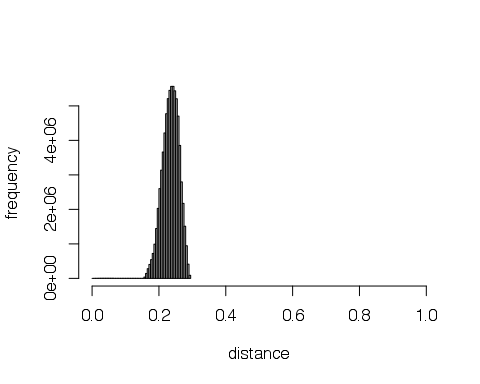
\includegraphics[scale=0.5]{figure/simtree_dist.png}}
     \subfloat[][UK]{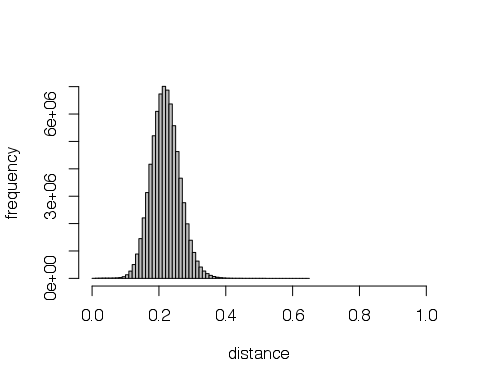
\includegraphics[scale=0.5]{figure/uktree_dist.png}}
     \caption{Distances (subst/site)}
\end{figure}

\begin{knitrout}
\definecolor{shadecolor}{rgb}{0.969, 0.969, 0.969}\color{fgcolor}\begin{kframe}
\begin{alltt}
\hlstd{detail_knitr} \hlkwb{<-} \hlnum{TRUE}
\hlkwd{source}\hlstd{(}\hlstr{"functions.R"}\hlstd{)}
\end{alltt}
\end{kframe}
\end{knitrout}

\begin{knitrout}
\definecolor{shadecolor}{rgb}{0.969, 0.969, 0.969}\color{fgcolor}\begin{kframe}
\begin{alltt}
\hlkwd{library}\hlstd{(ape)}
\end{alltt}


{\ttfamily\noindent\color{warningcolor}{Warning: package 'ape' was built under R version 3.2.3}}\begin{alltt}
\hlkwa{if}\hlstd{(}\hlnum{TRUE}\hlstd{)\{}
  \hlcom{####---- load sim ----}
  \hlcom{## Load newest Rdata}
  \hlstd{l} \hlkwb{<-} \hlkwd{list.files}\hlstd{(}\hlkwc{pattern}\hlstd{=}\hlstr{"*.Rdata"}\hlstd{)} \hlcom{# list.files(pattern="Rdata$") list.files(pattern="out")}
  \hlstd{l}
  \hlkwd{load}\hlstd{(l[}\hlkwd{length}\hlstd{(l)])}
  \hlkwd{ls}\hlstd{()}
  \hlstd{simtree} \hlkwb{<-} \hlstd{tree}
  \hlkwd{rm}\hlstd{(tree)}

  \hlcom{####---- load uk stuff ----}
  \hlstd{t_uk} \hlkwb{<-} \hlkwd{read.tree}\hlstd{(}\hlkwc{file} \hlstd{=} \hlstr{"../phylo-uk/data/ExaML_result.subUKogC_noDRM.finaltree.000"}\hlstd{)}
  \hlcom{## drop OG}
  \hlstd{og} \hlkwb{<-} \hlkwd{c}\hlstd{(}\hlstr{"Ref1"}\hlstd{,} \hlstr{"Ref2"}\hlstd{,} \hlstr{"Ref3"}\hlstd{,} \hlstr{"Ref4"}\hlstd{,} \hlstr{"Ref5"}\hlstd{,} \hlstr{"Ref6"}\hlstd{,} \hlstr{"HXB2"}\hlstd{)}
  \hlstd{uktree} \hlkwb{<-} \hlkwd{drop.tip}\hlstd{(t_uk, og )}
 \hlstd{\}}
\end{alltt}
\end{kframe}
\end{knitrout}





\begin{knitrout}
\definecolor{shadecolor}{rgb}{0.969, 0.969, 0.969}\color{fgcolor}\begin{kframe}
\begin{alltt}
\hlcom{## of (transformed) distances}
\hlkwa{if}\hlstd{(}\hlnum{FALSE}\hlstd{)\{}

  \hlcom{# function TReeToEdgeList returns path to RDS file}

  \hlcom{##- simtree}
  \hlkwd{system.time}\hlstd{(}
  \hlstd{path.simtree_el} \hlkwb{<-} \hlkwd{TreeToEdgeList}\hlstd{(}\hlkwc{t} \hlstd{= simtree,}
                       \hlkwc{rate} \hlstd{=} \hlnum{4.3e-3}\hlopt{/}\hlnum{365}\hlstd{,} \hlcom{# Berry et al. JVI 2007}
                       \hlkwc{seqlength} \hlstd{=} \hlnum{1550}\hlstd{)}
  \hlstd{)}

  \hlcom{##- uktree (no transformation)}
  \hlkwd{system.time}\hlstd{(}
    \hlstd{path.uktree_el} \hlkwb{<-} \hlkwd{TreeToEdgeList}\hlstd{(uktree,}
                        \hlkwc{rate} \hlstd{=} \hlnum{1}\hlstd{) )}
\hlstd{\}}


\hlcom{# Alternatively take TN93 distances}
\hlcom{#  dukTN93 <- readRDS(file = "../phylo-uk/source/subUKogC_noDRM_151202_ucsdTN93.rds" )}
\end{alltt}
\end{kframe}
\end{knitrout}

\begin{knitrout}
\definecolor{shadecolor}{rgb}{0.969, 0.969, 0.969}\color{fgcolor}\begin{kframe}
\begin{alltt}
\hlcom{## get list of quantiles, commands and list of}
\hlcom{## dataframes of cluster members }
\hlkwa{if}\hlstd{(}\hlnum{FALSE}\hlstd{)\{}
  \hlstd{thresholds} \hlkwb{=} \hlkwd{c}\hlstd{(}\hlnum{0.015}\hlstd{,} \hlnum{0.02}\hlstd{,} \hlnum{0.05}\hlstd{,} \hlnum{0.1}\hlstd{)}
  \hlkwd{system.time}\hlstd{(}
    \hlstd{simclus} \hlkwb{<-} \hlkwd{ucsd_hivclust}\hlstd{(}\hlkwc{path.el} \hlstd{= path.simtree_el,}
                             \hlkwc{thr} \hlstd{= thresholds)}
  \hlstd{)}

  \hlkwd{system.time}\hlstd{(}
    \hlstd{ukclus} \hlkwb{<-} \hlkwd{ucsd_hivclust}\hlstd{(}\hlkwc{path.el} \hlstd{= path.uktree_el,}
                            \hlkwc{thr} \hlstd{= thresholds)}
  \hlstd{)}
  \hlkwd{names}\hlstd{(simclus)}
  \hlkwd{names}\hlstd{(ukclus)}
  \hlcom{# unlist(ukclus["warn"] , recursive = T, use.names = F)}

  \hlcom{###--- save }
  \hlkwd{saveRDS}\hlstd{(simclus,} \hlkwc{file} \hlstd{=} \hlstr{"data/simclus2.rds"}\hlstd{)}
  \hlkwd{saveRDS}\hlstd{(ukclus,} \hlkwc{file} \hlstd{=} \hlstr{"data/ukclus2.rds"}\hlstd{)}
 \hlstd{\}}

\hlcom{# rm(dsimtree, duktree)}
\end{alltt}
\end{kframe}
\end{knitrout}


\section{UCSD hivclustering}
Read saved results from UCSD \textsf{hivclustering}
\begin{knitrout}
\definecolor{shadecolor}{rgb}{0.969, 0.969, 0.969}\color{fgcolor}\begin{kframe}
\begin{alltt}
\hlcom{### only cluster members (based on given threshold)}
\hlstd{simclus} \hlkwb{<-} \hlkwd{readRDS}\hlstd{(}\hlkwc{file} \hlstd{=} \hlstr{"data/simclus2.rds"}\hlstd{)[[}\hlstr{"cl"}\hlstd{]]}
\hlstd{ukclus} \hlkwb{<-} \hlkwd{readRDS}\hlstd{(}\hlkwc{file} \hlstd{=} \hlstr{"data/ukclus2.rds"}\hlstd{)[[}\hlstr{"cl"}\hlstd{]]}

\hlcom{### only cluster members (based on quantiles)}
\hlcom{# simclus <- readRDS(file = "data/simclus.rds")[[3]]}
\hlcom{# ukclus <- readRDS(file = "data/ukclus.rds")[[3]]}
\end{alltt}
\end{kframe}
\end{knitrout}
\begin{itemize}
\item Now, thresholds for clustering are fixed and not determined by quantiles of distances
\item Because of this and because of the applied substitution rate, the number of clusters and mean sizes of clusters are not identical but are of the same magnitude between simulated and real UK data
\item Up to threshold = 5\%, distributions of cluster size seem to follow a power law for both simulated and UK data 
\end{itemize}

Number of clusters and stats for simulated and UK trees (cluster size 1 does not exist in these (UCSD) outputs)
\begin{knitrout}
\definecolor{shadecolor}{rgb}{0.969, 0.969, 0.969}\color{fgcolor}\begin{kframe}
\begin{alltt}
\hlcom{##- Calculate size(=Freq) of each cluster across different threshold}
\hlstd{simfreqClust} \hlkwb{<-} \hlkwd{lapply}\hlstd{(simclus,}
                       \hlkwa{function}\hlstd{(}\hlkwc{x}\hlstd{)} \hlkwd{as.data.frame}\hlstd{(}\hlkwd{table}\hlstd{(x}\hlopt{$}\hlstd{ClusterID),}
                       \hlkwc{stringsAsFactors} \hlstd{=} \hlnum{FALSE}\hlstd{))}
\hlstd{ukfreqClust} \hlkwb{<-} \hlkwd{lapply}\hlstd{(ukclus,}
                      \hlkwa{function}\hlstd{(}\hlkwc{x}\hlstd{)} \hlkwd{as.data.frame}\hlstd{(}\hlkwd{table}\hlstd{(x}\hlopt{$}\hlstd{ClusterID),}
                      \hlkwc{stringsAsFactors} \hlstd{=} \hlnum{FALSE}\hlstd{))}
\end{alltt}
\end{kframe}
\end{knitrout}

\begin{knitrout}
\definecolor{shadecolor}{rgb}{0.969, 0.969, 0.969}\color{fgcolor}\begin{kframe}
\begin{alltt}
\hlcom{##- number of different clusters by threshold}
\hlkwd{sapply}\hlstd{(simfreqClust,} \hlkwa{function}\hlstd{(}\hlkwc{x}\hlstd{)} \hlkwd{dim}\hlstd{(x)[}\hlnum{1}\hlstd{])}
\end{alltt}
\begin{verbatim}
0.015  0.02  0.05   0.1 
 1713  2048  2006  1632 
\end{verbatim}
\begin{alltt}
\hlkwd{sapply}\hlstd{(ukfreqClust,} \hlkwa{function}\hlstd{(}\hlkwc{x}\hlstd{)} \hlkwd{dim}\hlstd{(x)[}\hlnum{1}\hlstd{])}
\end{alltt}
\begin{verbatim}
0.015  0.02  0.05   0.1 
 1199  1374  1460   611 
\end{verbatim}
\begin{alltt}
\hlcom{##- cluster size}
\hlkwd{sapply}\hlstd{(simfreqClust,} \hlkwa{function}\hlstd{(}\hlkwc{x}\hlstd{)} \hlkwd{summary}\hlstd{(x}\hlopt{$}\hlstd{Freq))}
\end{alltt}
\begin{verbatim}
         0.015   0.02   0.05    0.1
Min.     2.000  2.000  2.000  2.000
1st Qu.  2.000  2.000  2.000  2.000
Median   2.000  2.000  3.000  4.000
Mean     2.762  3.138  5.182  6.913
3rd Qu.  3.000  4.000  6.000  9.000
Max.    12.000 21.000 34.000 52.000
\end{verbatim}
\begin{alltt}
\hlkwd{sapply}\hlstd{(ukfreqClust,} \hlkwa{function}\hlstd{(}\hlkwc{x}\hlstd{)} \hlkwd{summary}\hlstd{(x}\hlopt{$}\hlstd{Freq))}
\end{alltt}
\begin{verbatim}
          0.015    0.02    0.05     0.1
Min.      2.000   2.000   2.000    2.00
1st Qu.   2.000   2.000   2.000    2.00
Median    2.000   2.000   3.000    3.00
Mean      3.188   3.531   5.442   17.84
3rd Qu.   3.000   3.000   4.000    4.00
Max.    101.000 121.000 166.000 7986.00
\end{verbatim}
\end{kframe}
\end{knitrout}


Plots of log(size) for UK and simulated clusters
\begin{knitrout}
\definecolor{shadecolor}{rgb}{0.969, 0.969, 0.969}\color{fgcolor}

{\centering 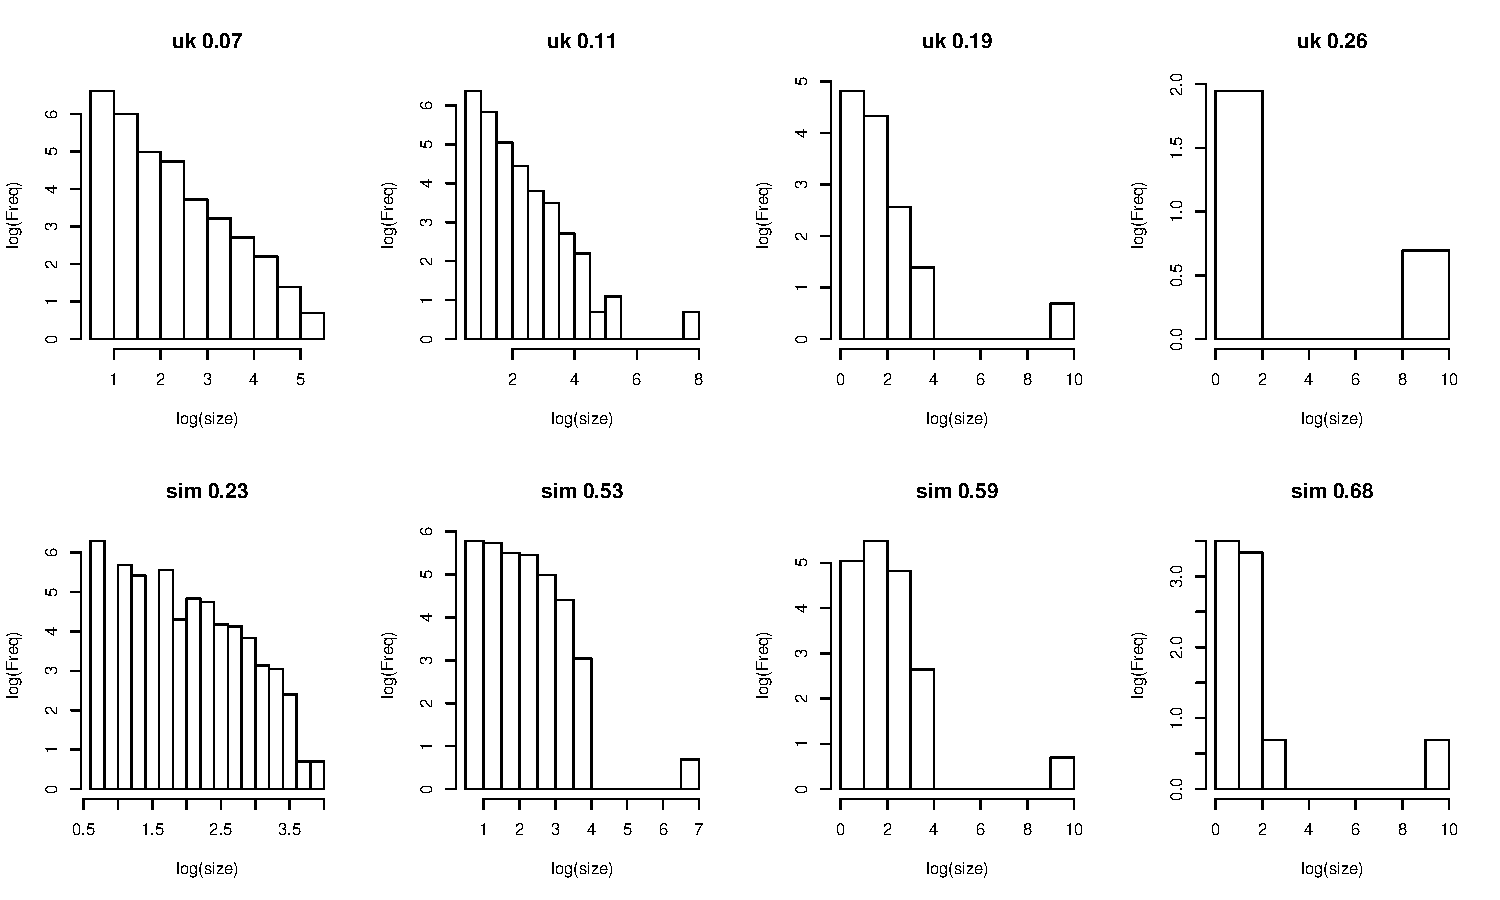
\includegraphics[width=11cm]{figure/plotplot_log-log-1} 

}



\end{knitrout}

QQ plots UK vs simulated, untransformed and log-log
\begin{knitrout}
\definecolor{shadecolor}{rgb}{0.969, 0.969, 0.969}\color{fgcolor}\begin{kframe}
\begin{verbatim}
null device 
          1 
\end{verbatim}
\end{kframe}

{\centering 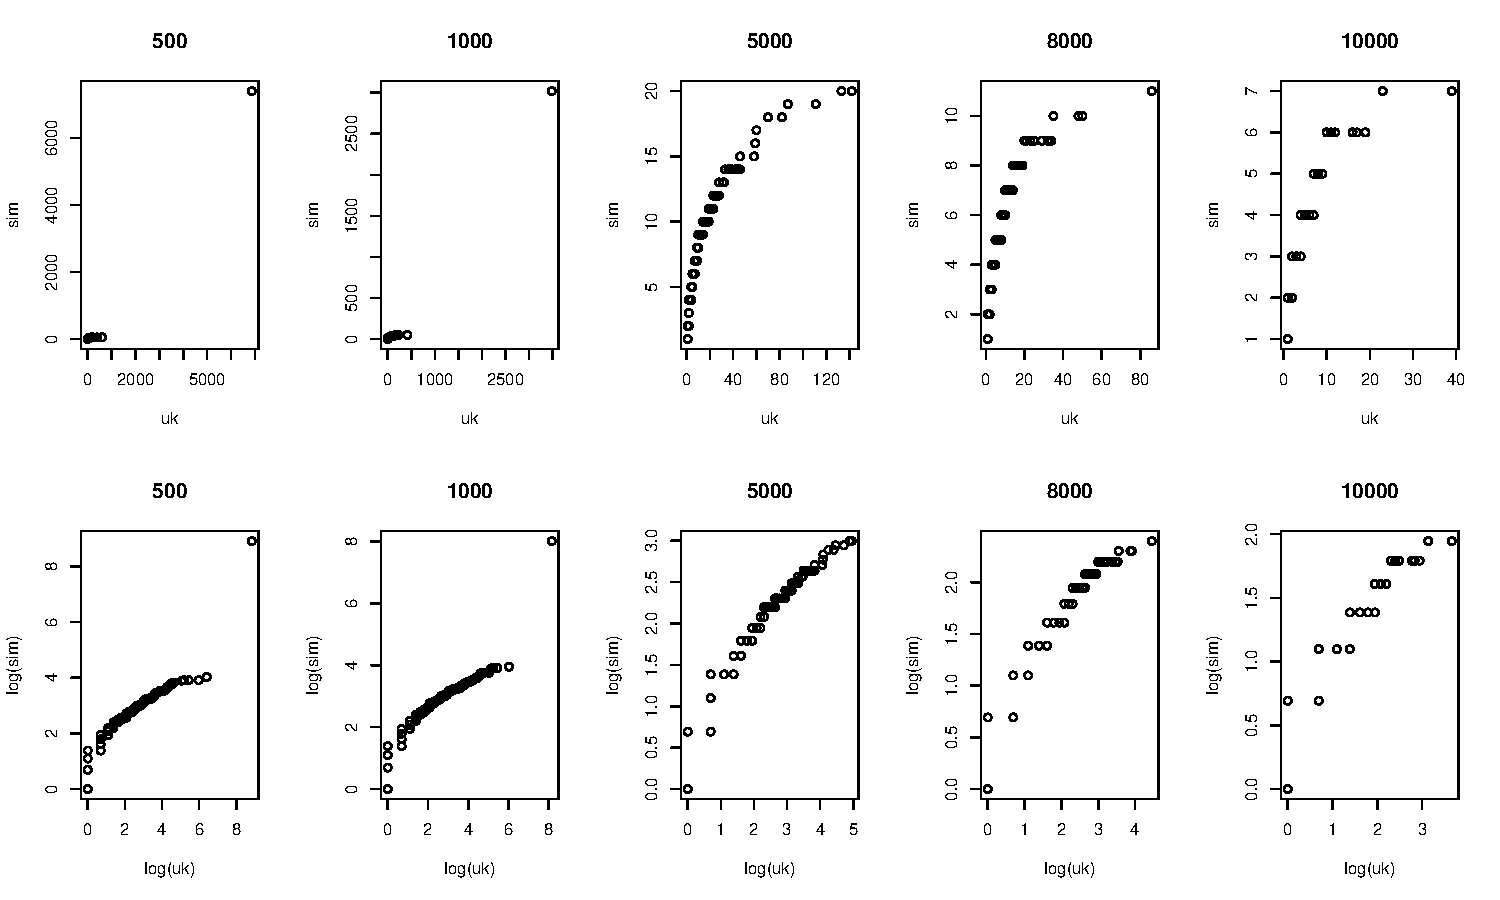
\includegraphics[width=11cm]{figure/plotQQ_plot-1} 

}



\end{knitrout}

\section{Associations}
After merging with co-variates allocated from demes states contained in tree, non-clustering individuals are assigned a cluster size of 1. 


The proportion of individuals into clusters (0 = out of, 1 = in a cluster) and stats for "size of cluster for each individuals". 
\begin{knitrout}
\definecolor{shadecolor}{rgb}{0.969, 0.969, 0.969}\color{fgcolor}\begin{kframe}
\begin{alltt}
\hlstd{demo} \hlkwb{<-} \hlkwd{readRDS}\hlstd{(}\hlstr{"demo.rds"}\hlstd{)}
\hlcom{##- date of diagnosis ?}
\hlstd{date0} \hlkwb{<-} \hlkwd{as.Date}\hlstd{(}\hlstr{'1979-01-01'}\hlstd{)}
\hlstd{demo}\hlopt{$}\hlstd{datediag} \hlkwb{<-} \hlstd{date0} \hlopt{+} \hlstd{demo}\hlopt{$}\hlstd{time}
\hlcom{# min(demo$datediag) head(demo)}
\hlcom{# max(demo$datediag)}

\hlcom{###--- add cluster sizes}
\hlcom{####... and outdegrees}
\end{alltt}
\end{kframe}
\end{knitrout}

\begin{knitrout}
\definecolor{shadecolor}{rgb}{0.969, 0.969, 0.969}\color{fgcolor}\begin{kframe}
\begin{alltt}
\hlcom{### --- start function clust.stats --- ###}
\hlcom{##- calculate both numclus and sizeclus for each seqindex into a LIST}
\hlcom{##- with same variable names}
\hlcom{##- For UCSD files, no ID if no cluster (size < 2) !}

\hlstd{clust.stats} \hlkwb{<-} \hlkwa{function}\hlstd{(}\hlkwc{clus} \hlstd{= simclus,} \hlkwc{tree} \hlstd{= simtree)\{}

  \hlcom{## get ALL tips names}
  \hlstd{tip.names} \hlkwb{<-} \hlkwd{data.frame}\hlstd{(}\hlstr{"id"} \hlstd{= tree}\hlopt{$}\hlstd{tip.label ,}
                          \hlkwc{stringsAsFactors} \hlstd{= F)}
  \hlcom{## get size of clusters}
  \hlstd{freqClust} \hlkwb{<-} \hlkwd{lapply}\hlstd{(clus,} \hlkwa{function}\hlstd{(}\hlkwc{x}\hlstd{)\{}
    \hlkwd{as.data.frame}\hlstd{(}\hlkwd{table}\hlstd{(x}\hlopt{$}\hlstd{ClusterID),}
                  \hlkwc{stringsAsFactors} \hlstd{=} \hlnum{FALSE}\hlstd{)}
  \hlstd{\})}

  \hlcom{## empty list}
  \hlstd{l} \hlkwb{<-} \hlkwd{list}\hlstd{()}

  \hlcom{## loop over thresholds}
  \hlkwa{for} \hlstd{(i} \hlkwa{in} \hlnum{1}\hlopt{:}\hlkwd{length}\hlstd{(clus) ) \{}
  \hlcom{## merge cluster number (with NA)}
   \hlstd{a} \hlkwb{<-} \hlkwd{merge}\hlstd{(}\hlkwc{x} \hlstd{= tip.names,} \hlkwc{y} \hlstd{= clus[[i]],}
          \hlkwc{by.x} \hlstd{=} \hlstr{"id"}\hlstd{,} \hlkwc{by.y} \hlstd{=} \hlstr{"SequenceID"}\hlstd{,}
          \hlkwc{all.x} \hlstd{=} \hlnum{TRUE}\hlstd{,} \hlkwc{sort} \hlstd{=} \hlnum{FALSE}\hlstd{)}

   \hlcom{## merge cluster size (with NA)}
   \hlstd{b} \hlkwb{<-} \hlkwd{merge}\hlstd{(}\hlkwc{x} \hlstd{= a,} \hlkwc{y} \hlstd{= freqClust[[i]],}
              \hlkwc{by.x} \hlstd{=} \hlstr{"ClusterID"}\hlstd{,} \hlkwc{by.y} \hlstd{=} \hlstr{"Var1"}\hlstd{,}
              \hlkwc{all.x} \hlstd{=} \hlnum{TRUE}\hlstd{,} \hlkwc{sort} \hlstd{=} \hlnum{FALSE}\hlstd{)}

  \hlcom{#- size 1 if not into a cluster}
  \hlstd{b}\hlopt{$}\hlstd{Freq[}\hlkwd{is.na}\hlstd{(b}\hlopt{$}\hlstd{Freq)]} \hlkwb{<-} \hlnum{1}

  \hlcom{#- binary clustering variable}
  \hlstd{b}\hlopt{$}\hlstd{binclus} \hlkwb{<-} \hlkwd{ifelse}\hlstd{(b}\hlopt{$}\hlstd{Freq} \hlopt{>} \hlnum{1} \hlopt{& !}\hlkwd{is.na}\hlstd{(b}\hlopt{$}\hlstd{Freq),} \hlnum{1}\hlstd{,} \hlnum{0}\hlstd{)}

  \hlcom{##- pseudo ClusterID when size = 1}
  \hlcom{## starting from max(ClusterID+1)}
  \hlcom{## important for down-sampling}
  \hlstd{.start} \hlkwb{<-} \hlkwd{max}\hlstd{(b}\hlopt{$}\hlstd{ClusterID,} \hlkwc{na.rm} \hlstd{= T)}
  \hlstd{.n} \hlkwb{<-} \hlkwd{dim}\hlstd{(b[}\hlkwd{is.na}\hlstd{(b}\hlopt{$}\hlstd{ClusterID),] )[}\hlnum{1}\hlstd{]}
   \hlstd{b}\hlopt{$}\hlstd{ClusterID[}\hlkwd{is.na}\hlstd{(b}\hlopt{$}\hlstd{ClusterID)]}  \hlkwb{<-} \hlstd{.start} \hlopt{+} \hlnum{1}\hlopt{:}\hlstd{.n}

  \hlcom{#- colnames}
  \hlkwd{colnames}\hlstd{(b)[}\hlkwd{which}\hlstd{(}\hlkwd{colnames}\hlstd{(b)} \hlopt{==}\hlstr{"Freq"}\hlstd{)]} \hlkwb{<-} \hlstr{"size"}
  \hlstd{l[[i]]} \hlkwb{<-} \hlstd{b}
  \hlkwd{names}\hlstd{(l)[i]} \hlkwb{<-} \hlkwd{names}\hlstd{(freqClust[i])}
  \hlstd{\}}
  \hlkwd{return}\hlstd{(l)}
\hlstd{\}}
\hlcom{### --- end function clust.stats --- ###}

\hlstd{l_sim} \hlkwb{<-}  \hlkwd{clust.stats}\hlstd{(}\hlkwc{clus} \hlstd{= simclus,} \hlkwc{tree} \hlstd{= simtree)}
\hlstd{l_uk} \hlkwb{<-}  \hlkwd{clust.stats}\hlstd{(}\hlkwc{clus} \hlstd{= ukclus,} \hlkwc{tree} \hlstd{= uktree)}
\hlcom{# str(l_sim)}
\hlcom{# str(l_uk)}
\end{alltt}
\end{kframe}
\end{knitrout}

\begin{knitrout}
\definecolor{shadecolor}{rgb}{0.969, 0.969, 0.969}\color{fgcolor}\begin{kframe}
\begin{alltt}
\hlcom{##- number of clusters (counting size=1 cluster !)}
\hlkwd{sapply}\hlstd{(l_sim,} \hlkwa{function}\hlstd{(}\hlkwc{x}\hlstd{)} \hlkwd{length}\hlstd{(}\hlkwd{unique}\hlstd{(x}\hlopt{$}\hlstd{ClusterID)))}
\end{alltt}
\begin{verbatim}
0.015  0.02  0.05   0.1 
 9146  7785  3774  2514 
\end{verbatim}
\begin{alltt}
\hlkwd{sapply}\hlstd{(l_uk,} \hlkwa{function}\hlstd{(}\hlkwc{x}\hlstd{)} \hlkwd{length}\hlstd{(}\hlkwd{unique}\hlstd{(x}\hlopt{$}\hlstd{ClusterID)))}
\end{alltt}
\begin{verbatim}
0.015  0.02  0.05   0.1 
 9541  8686  5679  1872 
\end{verbatim}
\begin{alltt}
\hlcom{##-proportion in or out clusters}
\hlkwd{sapply}\hlstd{(l_sim,} \hlkwa{function}\hlstd{(}\hlkwc{x}\hlstd{)} \hlkwd{round}\hlstd{(}\hlkwd{prop.table}\hlstd{(}\hlkwd{table}\hlstd{(x}\hlopt{$}\hlstd{binclus)),}\hlnum{2}\hlstd{))}
\end{alltt}
\begin{verbatim}
  0.015 0.02 0.05  0.1
0  0.61 0.47 0.15 0.07
1  0.39 0.53 0.85 0.93
\end{verbatim}
\begin{alltt}
\hlkwd{sapply}\hlstd{(l_uk,} \hlkwa{function}\hlstd{(}\hlkwc{x}\hlstd{)} \hlkwd{round}\hlstd{(}\hlkwd{prop.table}\hlstd{(}\hlkwd{table}\hlstd{(x}\hlopt{$}\hlstd{binclus)),}\hlnum{2}\hlstd{))}
\end{alltt}
\begin{verbatim}
  0.015 0.02 0.05 0.1
0  0.69  0.6 0.35 0.1
1  0.31  0.4 0.65 0.9
\end{verbatim}
\begin{alltt}
\hlcom{##- cluster sizes (by individuals having such a size !!)}
\hlcom{## probably meaningless}
\hlkwd{sapply}\hlstd{(l_sim,} \hlkwa{function}\hlstd{(}\hlkwc{x}\hlstd{)} \hlkwd{summary}\hlstd{(x}\hlopt{$}\hlstd{size))}
\end{alltt}
\begin{verbatim}
         0.015  0.02   0.05   0.1
Min.     1.000  1.00  1.000  1.00
1st Qu.  1.000  1.00  2.000  4.00
Median   1.000  2.00  6.000 10.00
Mean     1.951  2.74  7.949 12.29
3rd Qu.  2.000  3.00 11.000 17.00
Max.    12.000 21.00 34.000 52.00
\end{verbatim}
\begin{alltt}
\hlkwd{sapply}\hlstd{(l_uk,} \hlkwa{function}\hlstd{(}\hlkwc{x}\hlstd{)} \hlkwd{summary}\hlstd{(x}\hlopt{$}\hlstd{size))}
\end{alltt}
\begin{verbatim}
          0.015    0.02   0.05  0.1
Min.      1.000   1.000   1.00    1
1st Qu.   1.000   1.000   1.00   11
Median    1.000   1.000   3.00 7986
Mean      3.941   5.853  18.82 5247
3rd Qu.   2.000   3.000  16.00 7986
Max.    101.000 121.000 166.00 7986
\end{verbatim}
\end{kframe}
\end{knitrout}

\begin{knitrout}
\definecolor{shadecolor}{rgb}{0.969, 0.969, 0.969}\color{fgcolor}\begin{kframe}
\begin{alltt}
\hlcom{##- for simulated data}
\hlstd{listclus} \hlkwb{<-} \hlkwd{lapply}\hlstd{(l_sim,} \hlkwa{function}\hlstd{(}\hlkwc{x}\hlstd{)}
\hlkwd{merge}\hlstd{(x, demo,}
      \hlkwc{by.x} \hlstd{=} \hlstr{"id"}\hlstd{,} \hlkwc{by.y} \hlstd{=} \hlstr{"patient"}\hlstd{,}
      \hlkwc{all.x} \hlstd{= T,} \hlkwc{sort} \hlstd{=} \hlnum{FALSE}\hlstd{))}

\hlcom{# head(listclus[[3]])}
\hlcom{# table(listclus[[1]]$binclus, useNA = "ifany")}
\hlcom{# table(listclus[[1]]$size, useNA = "ifany")}
\hlcom{# saveRDS(listclus, file = "data/listclus_sim.rds")}

\hlcom{###########################}
\hlcom{### --- Regressions --- ###}
\hlcom{###########################}
\end{alltt}
\end{kframe}
\end{knitrout}

\subsection{Naive regressions on simulation}

Linear regression with co-variates as ordinal or categorical
\begin{knitrout}
\definecolor{shadecolor}{rgb}{0.969, 0.969, 0.969}\color{fgcolor}\begin{kframe}
\begin{alltt}
\hlcom{##- linear}
\hlstd{lm_model_factor} \hlkwb{<-} \hlstr{"size ~ factor(stage) + factor(risk) + factor(age)"}
\hlstd{lm_model_ordinal}  \hlkwb{<-}  \hlstr{"scale(size) ~ scale(age) + scale(stage) + scale(time) + scale(risk)"}
\hlstd{lm_model_ordinal_wo_time}  \hlkwb{<-}  \hlstr{"scale(size) ~ scale(age) + scale(stage) + scale(risk)"}

\hlcom{##- logistic}
\hlstd{logit_model_ord}  \hlkwb{<-}  \hlstr{"binclus ~ scale(age) + scale(stage) + scale(time) + scale(risk)"}
\hlstd{logit_model_fact} \hlkwb{<-}  \hlstr{"binclus ~ factor(stage) + factor(risk) + factor(age)"}

\hlcom{##- standard output}
\hlkwd{lapply}\hlstd{(listclus ,} \hlkwa{function}\hlstd{(}\hlkwc{x}\hlstd{)} \hlkwd{summary}\hlstd{(}\hlkwd{lm}\hlstd{(lm_model_ordinal,} \hlkwc{data} \hlstd{= x)))}
\end{alltt}
\begin{verbatim}
$`0.015`

Call:
lm(formula = lm_model_ordinal, data = x)

Residuals:
    Min      1Q  Median      3Q     Max 
-1.1738 -0.5708 -0.2452  0.1764  5.6731 

Coefficients:
               Estimate Std. Error t value Pr(>|t|)    
(Intercept)   2.591e-14  8.664e-03   0.000    1.000    
scale(age)   -3.771e-03  8.731e-03  -0.432    0.666    
scale(stage) -9.522e-02  8.737e-03 -10.899   <2e-16 ***
scale(time)   2.721e-01  8.698e-03  31.283   <2e-16 ***
scale(risk)  -1.263e-02  8.666e-03  -1.458    0.145    
---
Signif. codes:  0 '***' 0.001 '**' 0.01 '*' 0.05 '.' 0.1 ' ' 1

Residual standard error: 0.9555 on 12159 degrees of freedom
Multiple R-squared:  0.08723,	Adjusted R-squared:  0.08693 
F-statistic: 290.5 on 4 and 12159 DF,  p-value: < 2.2e-16


$`0.02`

Call:
lm(formula = lm_model_ordinal, data = x)

Residuals:
    Min      1Q  Median      3Q     Max 
-1.2970 -0.5903 -0.2302  0.2393  6.8647 

Coefficients:
               Estimate Std. Error t value Pr(>|t|)    
(Intercept)  -1.894e-15  8.605e-03   0.000    1.000    
scale(age)   -5.321e-03  8.672e-03  -0.614    0.540    
scale(stage) -8.114e-02  8.678e-03  -9.350   <2e-16 ***
scale(time)   2.984e-01  8.639e-03  34.535   <2e-16 ***
scale(risk)  -1.325e-02  8.607e-03  -1.540    0.124    
---
Signif. codes:  0 '***' 0.001 '**' 0.01 '*' 0.05 '.' 0.1 ' ' 1

Residual standard error: 0.9491 on 12159 degrees of freedom
Multiple R-squared:  0.09959,	Adjusted R-squared:  0.09929 
F-statistic: 336.2 on 4 and 12159 DF,  p-value: < 2.2e-16


$`0.05`

Call:
lm(formula = lm_model_ordinal, data = x)

Residuals:
    Min      1Q  Median      3Q     Max 
-1.5705 -0.6518 -0.3025  0.4489  4.3290 

Coefficients:
               Estimate Std. Error t value Pr(>|t|)    
(Intercept)  -5.295e-15  8.663e-03   0.000 1.000000    
scale(age)   -1.333e-02  8.730e-03  -1.527 0.126680    
scale(stage) -3.364e-02  8.736e-03  -3.851 0.000118 ***
scale(time)   2.885e-01  8.697e-03  33.176  < 2e-16 ***
scale(risk)  -3.042e-02  8.665e-03  -3.511 0.000448 ***
---
Signif. codes:  0 '***' 0.001 '**' 0.01 '*' 0.05 '.' 0.1 ' ' 1

Residual standard error: 0.9554 on 12159 degrees of freedom
Multiple R-squared:  0.0875,	Adjusted R-squared:  0.0872 
F-statistic: 291.5 on 4 and 12159 DF,  p-value: < 2.2e-16


$`0.1`

Call:
lm(formula = lm_model_ordinal, data = x)

Residuals:
    Min      1Q  Median      3Q     Max 
-1.5443 -0.6792 -0.2690  0.4122  4.3720 

Coefficients:
               Estimate Std. Error t value Pr(>|t|)    
(Intercept)   3.997e-15  8.804e-03   0.000   1.0000    
scale(age)   -4.255e-03  8.873e-03  -0.480   0.6315    
scale(stage) -2.563e-02  8.878e-03  -2.886   0.0039 ** 
scale(time)   2.351e-01  8.839e-03  26.594   <2e-16 ***
scale(risk)  -2.246e-02  8.806e-03  -2.550   0.0108 *  
---
Signif. codes:  0 '***' 0.001 '**' 0.01 '*' 0.05 '.' 0.1 ' ' 1

Residual standard error: 0.971 on 12159 degrees of freedom
Multiple R-squared:  0.05747,	Adjusted R-squared:  0.05716 
F-statistic: 185.4 on 4 and 12159 DF,  p-value: < 2.2e-16
\end{verbatim}
\begin{alltt}
\hlcom{####--- sim naive regressions ---}
\end{alltt}
\end{kframe}
\end{knitrout}

\begin{knitrout}
\definecolor{shadecolor}{rgb}{0.969, 0.969, 0.969}\color{fgcolor}\begin{kframe}
\begin{alltt}
\hlkwd{reg.sum}\hlstd{(}\hlkwc{ls} \hlstd{= listclus,} \hlkwc{reg} \hlstd{= lm,} \hlkwc{model} \hlstd{= lm_model_ordinal)}
\end{alltt}
\begin{verbatim}
$model
[1] "scale(size) ~ scale(age) + scale(stage) + scale(time) + scale(risk)"

$parameter
                0.015     0.02     0.05      0.1
(Intercept)   2.6e-14 -1.9e-15 -5.3e-15  4.0e-15
scale(age)   -3.8e-03 -5.3e-03 -1.3e-02 -4.3e-03
scale(stage) -9.5e-02 -8.1e-02 -3.4e-02 -2.6e-02
scale(time)   2.7e-01  3.0e-01  2.9e-01  2.4e-01
scale(risk)  -1.3e-02 -1.3e-02 -3.0e-02 -2.2e-02

$pvalue
             0.015 0.02 0.05 0.1
(Intercept)                     
scale(age)                      
scale(stage)   ***  ***  ***  **
scale(time)    ***  ***  *** ***
scale(risk)              ***   *

$r.squared
 0.015   0.02   0.05    0.1 
0.0872 0.0996 0.0875 0.0575 
\end{verbatim}
\begin{alltt}
\hlkwd{reg.sum}\hlstd{(}\hlkwc{ls} \hlstd{= listclus,} \hlkwc{reg} \hlstd{= lm,} \hlkwc{model} \hlstd{= lm_model_factor)}
\end{alltt}
\begin{verbatim}
$model
[1] "size ~ factor(stage) + factor(risk) + factor(age)"

$parameter
                0.015   0.02  0.05   0.1
(Intercept)     2.500  3.500  9.50 15.00
factor(stage)2 -0.370 -0.430 -0.74 -1.10
factor(stage)3 -0.400 -0.440 -0.53 -0.74
factor(stage)4 -0.570 -0.730 -1.10 -1.50
factor(stage)5 -0.710 -0.960 -1.40 -1.60
factor(risk)2  -0.057 -0.092 -0.54 -0.59
factor(age)2   -0.016 -0.150 -0.26 -0.91
factor(age)3   -0.170 -0.320 -0.94 -1.60
factor(age)4   -0.100 -0.250 -0.72 -1.10

$pvalue
               0.015 0.02 0.05 0.1
(Intercept)      ***  ***  *** ***
factor(stage)2   ***  ***  ***  **
factor(stage)3   ***  ***    *   *
factor(stage)4   ***  ***  *** ***
factor(stage)5   ***  ***  *** ***
factor(risk)2              ***   *
factor(age)2                     *
factor(age)3       *   **  *** ***
factor(age)4            *   **  **

$r.squared
  0.015    0.02    0.05     0.1 
0.01590 0.01270 0.00650 0.00453 
\end{verbatim}
\begin{alltt}
\hlcom{##- logistic}
\hlcom{##- model: clus ~ age +  stage + time + risk}
\hlcom{##- care = 1 for all at diagnosis}

\hlcom{# logfit <- lapply(simli , function(x)\{}
\hlcom{#   summary(glm(formula = logit_model_std, }
\hlcom{#               data = x, family = binomial(link = "logit")))}
\hlcom{#   \}) }
\end{alltt}
\end{kframe}
\end{knitrout}
\begin{itemize}
\item The size of cluster of each invidividuals is always explained by overall stage and time of sampling
\item For every threshold of clustering, stage 1 is more likely to belong to large clusters than any other stages
\item Age 1 is more likely to belong to large clusters than age 3 or age 4
\item Low (!) risk level is associated with larger clusters, only for higher thresholds (fewer and larger clusters on overall)
\item Small part of the variance is explained by the variables
\end{itemize}


Logistic regression with ordinal and categorical variables
\begin{knitrout}
\definecolor{shadecolor}{rgb}{0.969, 0.969, 0.969}\color{fgcolor}\begin{kframe}
\begin{alltt}
\hlkwd{reg.sum}\hlstd{(}\hlkwc{ls} \hlstd{= listclus,} \hlkwc{reg} \hlstd{= glm,} \hlkwc{model} \hlstd{= logit_model_ord,} \hlkwc{family} \hlstd{=} \hlkwd{binomial}\hlstd{(}\hlkwc{link} \hlstd{=} \hlstr{"logit"}\hlstd{))}
\end{alltt}
\begin{verbatim}
$model
[1] "binclus ~ scale(age) + scale(stage) + scale(time) + scale(risk)"

$parameter
              0.015   0.02   0.05   0.1
(Intercept)  -0.500  0.120  2.100  3.00
scale(age)   -0.043 -0.080 -0.065 -0.09
scale(stage) -0.260 -0.240 -0.160 -0.14
scale(time)   0.570  0.580  0.860  0.98
scale(risk)  -0.046 -0.053 -0.130 -0.13

$pvalue
             0.015 0.02 0.05 0.1
(Intercept)    ***  ***  *** ***
scale(age)       *  ***    *   *
scale(stage)   ***  ***  *** ***
scale(time)    ***  ***  *** ***
scale(risk)      *   **  *** ***
\end{verbatim}
\begin{alltt}
\hlkwd{reg.sum}\hlstd{(}\hlkwc{ls} \hlstd{= listclus,} \hlkwc{reg} \hlstd{= glm,} \hlkwc{model} \hlstd{= logit_model_fact,} \hlkwc{family} \hlstd{=} \hlkwd{binomial}\hlstd{(}\hlkwc{link} \hlstd{=} \hlstr{"logit"}\hlstd{))}
\end{alltt}
\begin{verbatim}
$model
[1] "binclus ~ factor(stage) + factor(risk) + factor(age)"

$parameter
                0.015  0.02  0.05   0.1
(Intercept)     0.290  1.00  2.40  3.50
factor(stage)2 -0.420 -0.42 -0.14 -0.24
factor(stage)3 -0.520 -0.46 -0.20 -0.18
factor(stage)4 -0.790 -0.75 -0.42 -0.48
factor(stage)5 -0.930 -0.91 -0.60 -0.60
factor(risk)2  -0.110 -0.13 -0.30 -0.30
factor(age)2   -0.054 -0.19 -0.17 -0.43
factor(age)3   -0.220 -0.38 -0.38 -0.62
factor(age)4   -0.230 -0.40 -0.37 -0.62

$pvalue
               0.015 0.02 0.05 0.1
(Intercept)      ***  ***  *** ***
factor(stage)2   ***  ***        .
factor(stage)3   ***  ***    *    
factor(stage)4   ***  ***  *** ***
factor(stage)5   ***  ***  *** ***
factor(risk)2      *   **  *** ***
factor(age)2            *        *
factor(age)3      **  ***   **  **
factor(age)4      **  ***   **  **
\end{verbatim}
\end{kframe}
\end{knitrout}
All variables are significantly associated with being into a cluster for all thresholds



\subsection{Regressions on down-sampled simulation}

\begin{itemize}
  \item For each clustering threshold, 
  \item sample one individual by cluster
  \item re-sample 100 times
  \item sample size equals number of clusters with each non-clustered individuals counting for one
    \begin{enumerate}
    \item First type of analysis
      \begin{itemize}
      \item apply 100 linear regressions on each sample
      \item calculate proportion of p-values < 0.05 over the 100 iterations
      
    

\begin{knitrout}
\definecolor{shadecolor}{rgb}{0.969, 0.969, 0.969}\color{fgcolor}\begin{kframe}
\begin{alltt}
\hlcom{### De-correlating: sample one individual by cluster. Repeat many times. Ensure much more power than downsampling with just one value per sample size.}
\hlkwd{head}\hlstd{(listclus[[}\hlnum{1}\hlstd{]])}
\end{alltt}
\begin{verbatim}
   id ClusterID size binclus  time age care stage risk   datediag
1  40      1520    3       1 12402   1    1     1    1 2012-12-15
2 211      1520    3       1 12311   4    1     5    1 2012-09-15
3  32      1520    3       1 12402   1    1     3    1 2012-12-15
4 611        40    2       1 12098   4    1     1    1 2012-02-15
5 440        40    2       1 12188   3    1     4    1 2012-05-15
6 964       430    2       1 11914   4    1     3    2 2011-08-15
\end{verbatim}
\begin{alltt}
\hlkwd{summary}\hlstd{(listclus[[}\hlnum{1}\hlstd{]]}\hlopt{$}\hlstd{size)} \hlcom{## contains size = 1}
\end{alltt}
\begin{verbatim}
   Min. 1st Qu.  Median    Mean 3rd Qu.    Max. 
  1.000   1.000   1.000   1.951   2.000  12.000 
\end{verbatim}
\begin{alltt}
\hlcom{###--- start function by threshold }
\hlcom{# df <- listclus[[1]]}

\hlstd{downsample} \hlkwb{<-} \hlkwa{function}\hlstd{(}\hlkwc{df}\hlstd{,} \hlkwc{lm_model} \hlstd{= lm_model,} \hlkwc{var} \hlstd{=} \hlkwd{c}\hlstd{(}\hlstr{"time"}\hlstd{,} \hlstr{"age"}\hlstd{,} \hlstr{"care"}\hlstd{,} \hlstr{"stage"}\hlstd{,} \hlstr{"risk"}\hlstd{),} \hlkwc{iter} \hlstd{=} \hlnum{2}\hlstd{)\{}
  \hlcom{##- sampling one id per cluster k times}
  \hlstd{k} \hlkwb{<-} \hlstd{iter}
  \hlcom{## loop}
    \hlcom{## empty list}
    \hlstd{down_listclus} \hlkwb{<-} \hlkwd{vector}\hlstd{(}\hlstr{"list"}\hlstd{, k)}
    \hlcom{##  k selection of one id from df}
    \hlcom{##   sampled by each ClusterID}
    \hlkwa{for} \hlstd{(i} \hlkwa{in} \hlnum{1}\hlopt{:}\hlstd{k)\{}
      \hlstd{down_listclus[[i]]} \hlkwb{<-} \hlstd{df[df}\hlopt{$}\hlstd{id} \hlopt
                                 \hlkwd{tapply}\hlstd{(df}\hlopt{$}\hlstd{id,}
                  \hlstd{df}\hlopt{$}\hlstd{ClusterID,}
                  \hlkwa{function}\hlstd{(}\hlkwc{x}\hlstd{)} \hlkwd{sample}\hlstd{(x,} \hlnum{1}\hlstd{)),]}
    \hlstd{\}}
  \hlcom{# head(down_listclus[[1]])}
  \hlcom{# dim(down_listclus[[1]])}

  \hlcom{##- linear regression for each iteration}
  \hlstd{fit} \hlkwb{<-} \hlkwd{lapply}\hlstd{(down_listclus,}
                \hlkwa{function}\hlstd{(}\hlkwc{x}\hlstd{)}
                  \hlkwd{summary}\hlstd{(}\hlkwd{lm}\hlstd{(lm_model,} \hlkwc{data} \hlstd{= x)))}

  \hlcom{##- extract coefficient}
    \hlcom{## number of variables + intercept}
    \hlstd{nvar} \hlkwb{<-} \hlkwd{dim}\hlstd{(}\hlkwd{coef}\hlstd{(fit[[}\hlnum{1}\hlstd{]]))[}\hlnum{1}\hlstd{]}

    \hlcom{## empty matrix of coefficients}
    \hlstd{coef_lm} \hlkwb{<-} \hlkwd{matrix}\hlstd{(}\hlnum{NA}\hlstd{, nvar} \hlopt{*} \hlstd{k,} \hlnum{4}\hlstd{,}
                  \hlkwc{dimnames} \hlstd{=} \hlkwd{list}\hlstd{(}
                    \hlkwd{rep}\hlstd{(}\hlkwd{rownames}\hlstd{(} \hlkwd{coef}\hlstd{(fit[[}\hlnum{1}\hlstd{]]) ), k),}
                    \hlkwd{colnames}\hlstd{(}\hlkwd{coef}\hlstd{(fit[[}\hlnum{1}\hlstd{]]))))}
    \hlcom{## loop}
    \hlkwa{for} \hlstd{(i} \hlkwa{in} \hlnum{1}\hlopt{:}\hlkwd{length}\hlstd{(fit))\{}
      \hlstd{fill} \hlkwb{<-} \hlstd{(i}\hlopt{-}\hlnum{1}\hlstd{)}\hlopt{*}\hlstd{nvar} \hlopt{+} \hlnum{1}\hlopt{:}\hlstd{nvar}
      \hlstd{coef_lm[ fill,  ]} \hlkwb{<-} \hlkwd{coef}\hlstd{(fit[[i]])}
    \hlstd{\}}

  \hlcom{##- number of p-value < 0.05}
  \hlstd{sum} \hlkwb{<-} \hlkwd{tapply}\hlstd{(coef_lm[,}\hlnum{4}\hlstd{],} \hlkwd{rownames}\hlstd{(coef_lm),}
                \hlkwa{function}\hlstd{(}\hlkwc{x}\hlstd{)} \hlkwd{sum}\hlstd{(x} \hlopt{<} \hlnum{0.05}\hlstd{)} \hlopt{/} \hlkwd{length}\hlstd{(x))}

  \hlcom{##- mean of co-variates over iterations}
  \hlcom{# head(down_listclus[[1]])}
    \hlcom{## change structure}
    \hlstd{bind_df} \hlkwb{<-} \hlkwd{do.call}\hlstd{(rbind, down_listclus)}
    \hlcom{## mean by ClusterID of set of variables var}
    \hlstd{mean.sample} \hlkwb{<-} \hlkwd{aggregate}\hlstd{(bind_df[, var],}
                           \hlkwd{list}\hlstd{(}\hlstr{"ClusterID"} \hlstd{= bind_df}\hlopt{$}\hlstd{ClusterID,}
                                \hlstr{"size"} \hlstd{= bind_df}\hlopt{$}\hlstd{size),                                                  mean)}

  \hlkwd{return}\hlstd{(}\hlkwd{list}\hlstd{(}\hlcom{# down_listclus = down_listclus,}
              \hlcom{#fit = fit, coef_lm = coef_lm,}
              \hlkwc{percent.signif} \hlstd{=  sum,} \hlkwc{mean.sample} \hlstd{= mean.sample))}
\hlstd{\}}
\end{alltt}
\end{kframe}
\end{knitrout}

\begin{knitrout}
\definecolor{shadecolor}{rgb}{0.969, 0.969, 0.969}\color{fgcolor}\begin{kframe}
\begin{alltt}
\hlcom{### over thresholds}

\hlcom{## ordinal variables}
  \hlstd{dd_ord} \hlkwb{<-} \hlkwd{sapply}\hlstd{( listclus,} \hlkwa{function}\hlstd{(}\hlkwc{x}\hlstd{) \{}
    \hlkwd{downsample}\hlstd{(}\hlkwc{df} \hlstd{= x,}
               \hlkwc{lm_model} \hlstd{= lm_model_ordinal,}
               \hlkwc{var} \hlstd{=} \hlkwd{c}\hlstd{(}\hlstr{"time"}\hlstd{,} \hlstr{"age"}\hlstd{,} \hlstr{"care"}\hlstd{,} \hlstr{"stage"}\hlstd{,} \hlstr{"risk"}\hlstd{),}
               \hlkwc{iter} \hlstd{=} \hlnum{100}\hlstd{)}
  \hlstd{\}}
  \hlstd{)}
  \hlcom{## percent of signif paramater}
  \hlkwd{t}\hlstd{(}\hlkwd{do.call}\hlstd{(rbind, dd_ord[}\hlstr{"percent.signif"}\hlstd{, ] ))}
\end{alltt}
\begin{verbatim}
             0.015 0.02 0.05  0.1
(Intercept)   0.00 0.00 0.00 0.00
scale(age)    0.22 0.43 0.13 0.09
scale(risk)   0.20 0.26 0.48 0.31
scale(stage)  1.00 1.00 0.75 0.62
scale(time)   1.00 1.00 1.00 1.00
\end{verbatim}
\begin{alltt}
\hlcom{## categorical variables}
  \hlstd{dd_cat} \hlkwb{<-} \hlkwd{sapply}\hlstd{( listclus,} \hlkwa{function}\hlstd{(}\hlkwc{x}\hlstd{) \{}
    \hlkwd{downsample}\hlstd{(}\hlkwc{df} \hlstd{= x,}
               \hlkwc{lm_model} \hlstd{= lm_model_factor,}
               \hlkwc{var} \hlstd{=} \hlkwd{c}\hlstd{(}\hlstr{"time"}\hlstd{,} \hlstr{"age"}\hlstd{,} \hlstr{"care"}\hlstd{,} \hlstr{"stage"}\hlstd{,} \hlstr{"risk"}\hlstd{),}
               \hlkwc{iter} \hlstd{=} \hlnum{100}\hlstd{)}
  \hlstd{\}}
  \hlstd{)}
  \hlcom{## percent of signif paramater}
  \hlkwd{t}\hlstd{(}\hlkwd{do.call}\hlstd{(rbind, dd_cat[}\hlstr{"percent.signif"}\hlstd{, ] ))}
\end{alltt}
\begin{verbatim}
               0.015 0.02 0.05  0.1
(Intercept)     1.00 1.00 1.00 1.00
factor(age)2    0.10 0.13 0.09 0.14
factor(age)3    0.34 0.65 0.38 0.35
factor(age)4    0.28 0.69 0.36 0.37
factor(risk)2   0.28 0.30 0.57 0.42
factor(stage)2  1.00 0.98 0.28 0.17
factor(stage)3  1.00 0.99 0.25 0.12
factor(stage)4  1.00 1.00 0.80 0.60
factor(stage)5  1.00 1.00 0.98 0.78
\end{verbatim}
\end{kframe}
\end{knitrout}

    \item For first two threshold, first stage of infection and recent time of sampling are always (100\%) associated with cluster size
    \item As sizes of clusters increase, young age and low-risk tend to be associated with cluster size (in maximum 47\% and 63\% of samples respectively)
  \end{itemize}

\item Second type of analysis
      \begin{itemize}
      \item calculate the mean of co-variates over the 100 iterations
      \item apply one linear regression: size ~ mean(covariates)
      \end{itemize}
    \end{enumerate}
\end{itemize}

\begin{knitrout}
\definecolor{shadecolor}{rgb}{0.969, 0.969, 0.969}\color{fgcolor}\begin{kframe}
\begin{alltt}
  \hlcom{## mean of co-variates by cluster}
  \hlcom{# str(dd["mean.sample",])}
  \hlstd{mean.down} \hlkwb{<-} \hlstd{dd_ord[}\hlstr{"mean.sample"}\hlstd{,]}

  \hlcom{##- linear regression ordinal}
\hlcom{#    lapply(mean.down, function(x) \{}
\hlcom{#    summary(lm(lm_model_ordinal, data = x))\})}
  \hlkwd{reg.sum}\hlstd{(}\hlkwc{ls} \hlstd{= mean.down,} \hlkwc{reg} \hlstd{= lm,} \hlkwc{model} \hlstd{= lm_model_ordinal)}
\end{alltt}
\begin{verbatim}
$model
[1] "scale(size) ~ scale(age) + scale(stage) + scale(time) + scale(risk)"

$parameter
                0.015     0.02     0.05      0.1
(Intercept)  -2.5e-14  2.6e-14  5.1e-15  1.0e-14
scale(age)   -1.2e-02 -2.0e-02 -1.4e-02 -1.4e-02
scale(stage) -8.1e-02 -8.2e-02 -4.6e-02 -5.2e-02
scale(time)   1.8e-01  2.0e-01  3.1e-01  3.5e-01
scale(risk)  -1.4e-02 -1.8e-02 -3.3e-02 -3.2e-02

$pvalue
             0.015 0.02 0.05 0.1
(Intercept)                     
scale(age)            .         
scale(stage)   ***  ***   **  **
scale(time)    ***  ***  *** ***
scale(risk)                *   .

$r.squared
 0.015   0.02   0.05    0.1 
0.0398 0.0487 0.1030 0.1290 
\end{verbatim}
\begin{alltt}
  \hlcom{## plot}
  \hlkwd{size.vs.covar}\hlstd{(mean.down)}
  \hlcom{# dev.off()}
\end{alltt}
\end{kframe}

{\centering 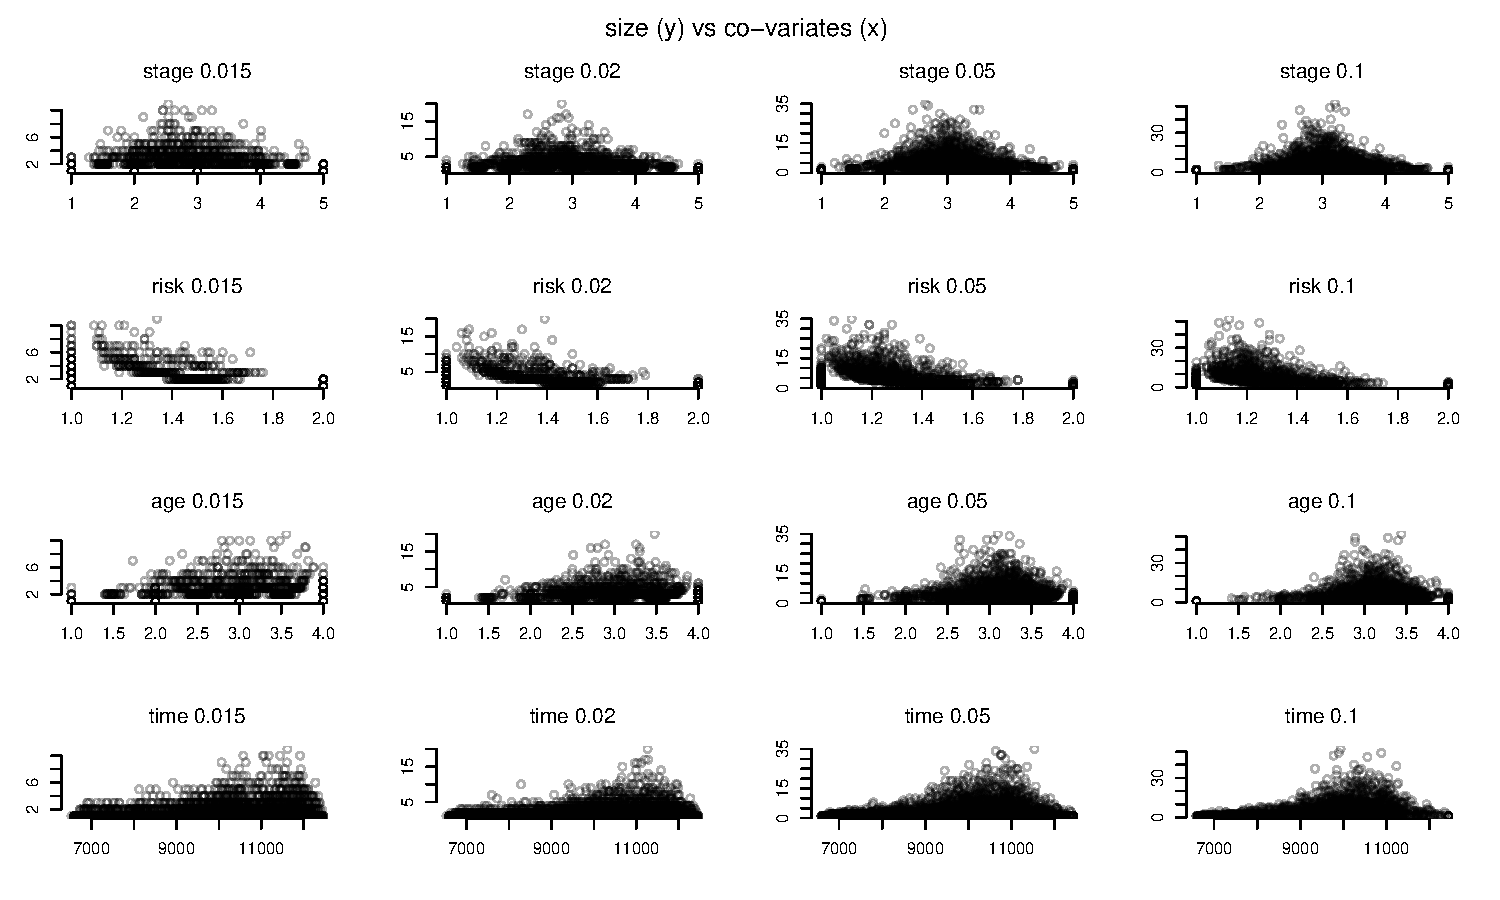
\includegraphics[width=11cm]{figure/plotrun_down-sample_2-1} 

}



\end{knitrout}
 \begin{itemize}
\item First stages of infection and recent time of sampling are always (100\%) associated with larger cluster size
 \end{itemize}
 
\subsection{On real UK data}
Same process ...
\begin{knitrout}
\definecolor{shadecolor}{rgb}{0.969, 0.969, 0.969}\color{fgcolor}\begin{kframe}
\begin{alltt}
\hlcom{##- add demo outcome: stage of infection, treatment status, age group, CHIC or not}
\hlkwd{load}\hlstd{(}\hlstr{"../phylo-uk/data/sub.RData"}\hlstd{)}
\hlkwd{rm}\hlstd{(s)}
\hlcom{##- selection of df covariates}
\hlstd{y} \hlkwb{<-} \hlstd{df[,}\hlkwd{c}\hlstd{(}\hlstr{"seqindex"}\hlstd{,}\hlstr{"patientindex"}\hlstd{,}
           \hlstr{"agediag"}\hlstd{,} \hlstr{"cd4"}\hlstd{,} \hlstr{"vl"}\hlstd{,} \hlstr{"onartflag"}\hlstd{,}
           \hlstr{"ydiag"}\hlstd{,} \hlstr{"agediag_cut"}\hlstd{,} \hlstr{"cd4cut"}\hlstd{,}
           \hlstr{"ydiag_cut"}\hlstd{,} \hlstr{"CHICflag"}\hlstd{,} \hlstr{"status"}\hlstd{)]}

\hlstd{y}\hlopt{$}\hlstd{logvl} \hlkwb{<-} \hlkwd{log}\hlstd{(y}\hlopt{$}\hlstd{vl)}
\hlstd{y}\hlopt{$}\hlstd{sqrtcd4} \hlkwb{<-} \hlkwd{sqrt}\hlstd{(y}\hlopt{$}\hlstd{cd4)}
\end{alltt}
\end{kframe}
\end{knitrout}

\begin{knitrout}
\definecolor{shadecolor}{rgb}{0.969, 0.969, 0.969}\color{fgcolor}\begin{kframe}
\begin{alltt}
\hlstd{listUKclus} \hlkwb{<-} \hlkwd{lapply}\hlstd{(l_uk,} \hlkwa{function}\hlstd{(}\hlkwc{x}\hlstd{)}
  \hlkwd{merge}\hlstd{(x, y,}
        \hlkwc{by.x} \hlstd{=} \hlstr{"id"}\hlstd{,} \hlkwc{by.y} \hlstd{=} \hlstr{"seqindex"}\hlstd{,}
        \hlkwc{all.x} \hlstd{= T,} \hlkwc{sort} \hlstd{=} \hlnum{FALSE}\hlstd{))}
\hlcom{# head(listUKclus[[1]])}

\hlcom{####--- naive regressions ---}
\end{alltt}
\end{kframe}
\end{knitrout}

\subsubsection{Naive regressions for real UK data}
Linear regression
\begin{knitrout}
\definecolor{shadecolor}{rgb}{0.969, 0.969, 0.969}\color{fgcolor}\begin{kframe}
\begin{alltt}
\hlcom{#### just on low and high threshold (but not too high !)}
\hlcom{# li <- listUKclus[ 1:(length(listUKclus)-1) ]}
\hlstd{lm_model_uk} \hlkwb{=} \hlstr{"scale(size) ~ scale(agediag) + scale(sqrt(cd4)) +  scale(ydiag)"}
\hlcom{# lapply(li, function(x) summary(lm(lm_model_std, data = x)))}
\hlkwd{reg.sum}\hlstd{(}\hlkwc{ls} \hlstd{= listUKclus,} \hlkwc{reg} \hlstd{= lm,} \hlkwc{model} \hlstd{= lm_model_uk)}
\end{alltt}
\begin{verbatim}
$model
[1] "scale(size) ~ scale(agediag) + scale(sqrt(cd4)) +  scale(ydiag)"

$parameter
                   0.015    0.02    0.05     0.1
(Intercept)       0.0022  0.0021  0.0024  0.0013
scale(agediag)   -0.0390 -0.0530 -0.0072  0.0970
scale(sqrt(cd4))  0.0380  0.0490  0.0480  0.0130
scale(ydiag)      0.1200  0.1500  0.1100 -0.2500

$pvalue
                 0.015 0.02 0.05 0.1
(Intercept)                         
scale(agediag)     ***  ***      ***
scale(sqrt(cd4))   ***  ***  ***    
scale(ydiag)       ***  ***  *** ***

$r.squared
 0.015   0.02   0.05    0.1 
0.0146 0.0234 0.0134 0.0583 
\end{verbatim}
\end{kframe}
\end{knitrout}
Young age, high level of CD4 and recent time of diagnosis are associated with larger cluster size
\begin{knitrout}
\definecolor{shadecolor}{rgb}{0.969, 0.969, 0.969}\color{fgcolor}\begin{kframe}
\begin{alltt}
\hlcom{##- model: clus ~ age +  stage + time + risk}
\hlcom{##- care = 1 for all at diagnosis}
\hlcom{## ex. }
\hlstd{logit_model_uk} \hlkwb{=} \hlstr{"binclus ~ scale(agediag) + scale(sqrt(cd4)) + scale(ydiag)"}

\hlkwd{reg.sum}\hlstd{(}\hlkwc{ls} \hlstd{= listUKclus,} \hlkwc{reg} \hlstd{= glm,} \hlkwc{model} \hlstd{= logit_model_uk,} \hlkwc{family} \hlstd{=} \hlkwd{binomial}\hlstd{(}\hlkwc{link} \hlstd{=} \hlstr{"logit"}\hlstd{))}
\end{alltt}
\begin{verbatim}
$model
[1] "binclus ~ scale(agediag) + scale(sqrt(cd4)) + scale(ydiag)"

$parameter
                 0.015  0.02  0.05     0.1
(Intercept)      -0.88 -0.47  0.71  2.2000
scale(agediag)   -0.17 -0.19 -0.14  0.0980
scale(sqrt(cd4))  0.22  0.22  0.25  0.2000
scale(ydiag)      0.73  0.75  0.72 -0.0032

$pvalue
                 0.015 0.02 0.05 0.1
(Intercept)        ***  ***  *** ***
scale(agediag)     ***  ***  ***  **
scale(sqrt(cd4))   ***  ***  *** ***
scale(ydiag)       ***  ***  ***    
\end{verbatim}
\end{kframe}
\end{knitrout}
Same associations with binary cluster membership

\subsubsection{Down-sampled regressions for real UK data}
\begin{knitrout}
\definecolor{shadecolor}{rgb}{0.969, 0.969, 0.969}\color{fgcolor}\begin{kframe}
\begin{alltt}
\hlcom{### over thresholds}

\hlcom{## ordinal variables}
\hlstd{dd_ord_uk} \hlkwb{<-} \hlkwd{sapply}\hlstd{( listUKclus,} \hlkwa{function}\hlstd{(}\hlkwc{x}\hlstd{) \{}
  \hlkwd{downsample}\hlstd{(}\hlkwc{df} \hlstd{= x,}
             \hlkwc{lm_model} \hlstd{= lm_model_uk,}
             \hlkwc{var} \hlstd{=} \hlkwd{c}\hlstd{(}\hlstr{"agediag"}\hlstd{,} \hlstr{"cd4"}\hlstd{,} \hlstr{"ydiag"}\hlstd{),}
             \hlkwc{iter} \hlstd{=} \hlnum{100}\hlstd{)}
\hlstd{\}}
\hlstd{)}
\hlcom{## percent of signif paramater}
\hlkwd{t}\hlstd{(}\hlkwd{do.call}\hlstd{(rbind, dd_ord_uk[}\hlstr{"percent.signif"}\hlstd{, ] ))}
\end{alltt}
\begin{verbatim}
                 0.015 0.02 0.05  0.1
(Intercept)       0.00 0.00 0.00 0.02
scale(agediag)    0.63 0.60 0.13 0.04
scale(sqrt(cd4))  0.85 0.92 0.76 0.07
scale(ydiag)      1.00 1.00 1.00 0.10
\end{verbatim}
\end{kframe}
\end{knitrout}

\begin{knitrout}
\definecolor{shadecolor}{rgb}{0.969, 0.969, 0.969}\color{fgcolor}\begin{kframe}
\begin{alltt}
\hlcom{## mean of co-variates by cluster}
\hlcom{# str(dd["mean.sample",])}
\hlstd{mean.down_uk} \hlkwb{<-} \hlstd{dd_ord_uk[}\hlstr{"mean.sample"}\hlstd{,]}
\hlcom{# head(mean.down_uk[[2]])}
\hlcom{##- linear regression ordinal}
\hlcom{#    lapply(mean.down, function(x) \{}
\hlcom{#    summary(lm(lm_model_ordinal, data = x))\})}
\hlkwd{reg.sum}\hlstd{(}\hlkwc{ls} \hlstd{= mean.down_uk,} \hlkwc{reg} \hlstd{= lm,} \hlkwc{model} \hlstd{= lm_model_uk)}
\end{alltt}
\begin{verbatim}
$model
[1] "scale(size) ~ scale(agediag) + scale(sqrt(cd4)) +  scale(ydiag)"

$parameter
                  0.015   0.02    0.05      0.1
(Intercept)      -0.018 -0.022 -0.0450 -2.4e-02
scale(agediag)   -0.017 -0.020 -0.0094 -8.5e-05
scale(sqrt(cd4))  0.034  0.038  0.0420  1.4e-03
scale(ydiag)      0.074  0.080  0.0730  1.9e-03

$pvalue
                 0.015 0.02 0.05 0.1
(Intercept)         **    *  *** ***
scale(agediag)       *    *         
scale(sqrt(cd4))   ***  ***  ***  **
scale(ydiag)       ***  ***  *** ***

$r.squared
 0.015   0.02   0.05    0.1 
0.0162 0.0121 0.0131 0.0170 
\end{verbatim}
\begin{alltt}
\hlcom{## plot}
\hlkwd{size.vs.covar}\hlstd{(}\hlkwc{l} \hlstd{= mean.down_uk,} \hlkwc{depvar} \hlstd{=} \hlstr{"size"}\hlstd{,}
\hlkwc{indepvar} \hlstd{=} \hlkwd{c}\hlstd{(}\hlstr{"agediag"}\hlstd{,} \hlstr{"cd4"}\hlstd{,} \hlstr{"ydiag"}\hlstd{))}
\hlcom{# dev.off()}
\end{alltt}
\end{kframe}

{\centering 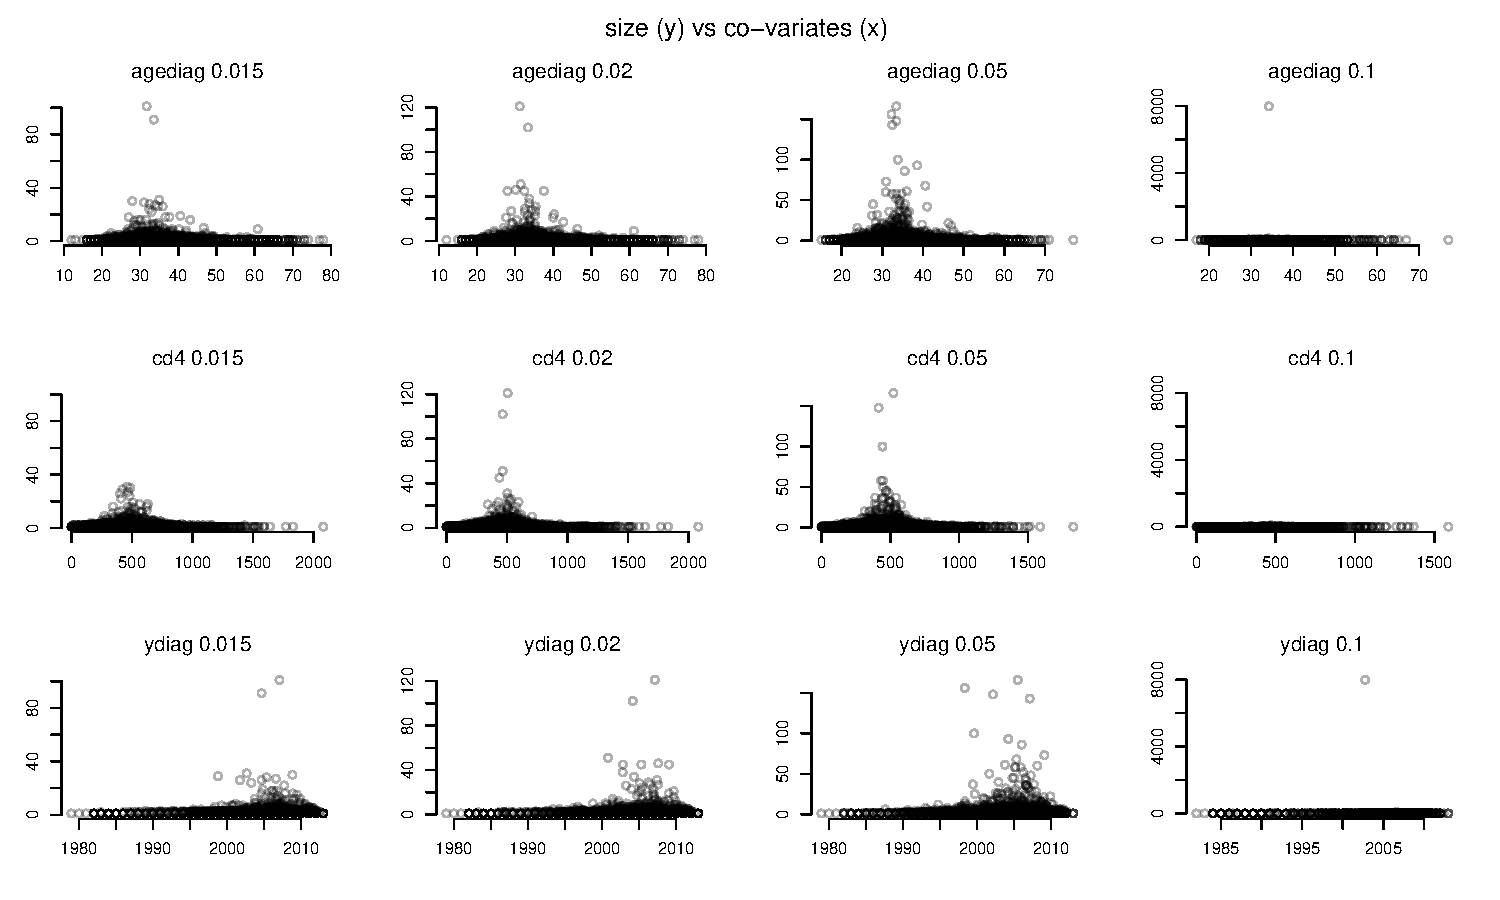
\includegraphics[width=11cm]{figure/plotrun_down-sample_UK_2-1} 

}



\end{knitrout}
CD4 and year of diagnosis systematically associated with cluster size / membership. 

\end{document}
